\Aufgabe[e]{Harmonischer Oszillator mit Resonanz}
{
Man betrachte die Differentialgleichung des harmonischen Oszillators
\[
y'' + 2\rho y' + \omega^2 y = r(t), \quad \text{mit } \rho, \omega \in \mathbb R_+
\]
mit den drei Fällen
\begin{enumerate}
  \item \textbf{Überdämpft (\( \rho > \omega \)):} Das System kehrt ohne Oszillation langsam zum Gleichgewicht zurück.
  $$
  r(t) = \operatorname{e}^{(-\rho + \sqrt{\rho^2 - \omega^2})t}
  $$
  \item \textbf{Kritisch gedämpft (\( \rho = \omega \)):} Das System kehrt so schnell wie möglich ohne Oszillation zum Gleichgewicht zurück mit
  $$
  r(t) = \operatorname{e}^{-\omega t}
  $$
  \item \textbf{Untergedämpft (\( \rho < \omega \)):} Das System oszilliert mit einer Amplitude, die allmählich auf null abnimmt.
  $$
  r(t) = \operatorname{e}^{-\rho t} \cos(\sqrt{\omega^2 - \rho^2}t)
  $$
\end{enumerate}
Bestimmen Sie die Lösung der Dgl. für die Fälle überdämpft, kritisch gedämpft und untergedämpft.
}


\Loesung{
\textbf{Fall 1: Überdämpft (\(\rho > \omega\))}

Die Wurzeln sind reell und unterschiedlich:
\[
\lambda = -\rho \pm \sqrt{\rho^2 - \omega^2}
\]
mit der homogenen Lösung:
\[
y_h(t) = A\operatorname{e}^{(-\rho + \sqrt{\rho^2 - \omega^2})t} + B\operatorname{e}^{(-\rho - \sqrt{\rho^2 - \omega^2})t}
\]
Wir führen die Abkürzung $z = \sqrt{\rho^2 - \omega^2}$ ein.
Für die partikuläre Lösung wählen wir den Ansatz
$$
y_p = A t \operatorname{e}^{(-\rho + z)t}.
$$
mit den Ableitungen
\begin{align*}
y_p' &= A ( 1+t(-\rho + z)) \operatorname{e}^{(-\rho + z)t}\\
y_p'' &= A (-\rho +z) ( 2+ t(-\rho +z)) \operatorname{e}^{(-\rho+z)t}
\end{align*}
Durch Einsetzen und Zusammenfassen erhalten wir
$$
2A\sqrt{\rho^2 -\omega^2} \operatorname{e}^{(-\rho+ \sqrt{\rho^2 - \omega^2})t} = \operatorname{e}^{(-\rho + \sqrt{\rho^2 - \omega^2})t}
$$
Damit ist $A= \frac{1}{2\sqrt{\rho^2-\omega^2}}$.
Die partikuläre Lösung ist
$$
y_p = \frac{1}{2\sqrt{\rho^2 -\omega^2}}t \operatorname{e}^{(-\rho +  \sqrt{\rho^2 - \omega^2})t}.
$$
Damit ist die allgemeine Lösung 
\begin{align*}
y = A\operatorname{e}^{(-\rho + \sqrt{\rho^2 - \omega^2})t} + B\operatorname{e}^{(-\rho - \sqrt{\rho^2 - \omega^2})t} + \frac{1}{2\sqrt{\rho^2 -\omega^2}}t \operatorname{e}^{(-\rho +  \sqrt{\rho^2 - \omega^2})t}.
\end{align*}


\begin{figure}[h]
    \centering
    \includegraphics[width=0.6\textwidth]{ueberdaempfterHarOszil.eps}
\end{figure}

\noindent
\textbf{Fall 2: Kritische Dämpfung (\(\rho = \omega\))} \\
Die charakteristische Gleichung vereinfacht sich zu:
\[
\lambda^2 + 2\omega \lambda + \omega^2 = 0
\]
mit einer doppelten Wurzel \(\lambda = -\omega\). Die homogene Lösung ist:
\[
y_h(t) =(A+Bt) \operatorname{e}^{-\omega t}.
\]
Da $\lambda = -\omega$ eine doppelte Nullstelle ist, wählen wir für die partikuläre 
Lösung den Ansatz
$$
y_p = At^2 \operatorname{e}^{-\omega t}.
$$
Wir bilden die Ableitungen
\begin{align*}
y_p' &= A\operatorname{e}^{-\omega t}(2t - \omega t^2)\\
y_p''& = A\operatorname{e}^{-\omega t}(2 +\omega^2t^2 - 4\omega t)
\end{align*}
Durch Einsetzen erhalten wir
\begin{align*}
\operatorname{e}^{-\omega t} &= 
A\operatorname{e}^{-\omega t} (2 + \omega^2 t^2 + 2\omega(2t- \omega t^2) + \omega^2 t^2)\\
&= 2A\operatorname{e}^{-\omega t}
\end{align*}
Damit ist $A = \frac{1}{2}$.
Die partikuläre Lösung ist
$$
y_p = \frac{1}{2}t^2 \operatorname{e}^{-\omega t}.
$$
Die allgemeine Lösung ist
$$
y = (A+Bt) \operatorname{e}^{-\omega t} + \frac{1}{2}t^2 \operatorname{e}^{-\omega t}.
$$

\begin{figure}[h]
    \centering
    \includegraphics[width=0.6\textwidth]{kritischegedaempfterHarOszil.eps}
\end{figure}

\noindent
\textbf{Fall 3: Untergedämpft (\(\rho < \omega\))} \\
Die Wurzeln sind komplex:
\[
\lambda = -\rho \pm i\sqrt{\omega^2 - \rho^2}
\]
was zu der homogenen Lösung führt:
\[
y_h(t) = \operatorname{e}^{-\rho t}(A \cos(\sqrt{\omega^2 - \rho^2} t) + B \sin(\sqrt{\omega^2 - \rho^2} t))
\]
Wir führen die Abkürzung $z = \sqrt{\omega^2 - \rho^2}$ ein.
Für die partikuläre Lösung wählen wir den Ansatz
$$
y_p = t\operatorname{e}^{-\rho t}(A\sin(zt) + B\cos(zt)) 
$$
Die Ableitungen sind
\begin{align*}
y_p' &= \operatorname{e}^{-\rho t}((A- \rho t A - ztB)\sin(zt) + (B-\rho t B + ztA) \cos(zt))\\
y_p'' &= \operatorname{e}^{-\rho t}( (-2\rho A - 2zB + t(2\rho zB + \rho^2 A -z^2A)) \sin(zt) \\
&+
          (-2\rho B +2zA + t(-2\rho zA + \rho^2 B - z^2B)) \cos(zt))
\end{align*}
Wir setzen die Ableitungen in die Differentialgleichung ein und erhalten
\begin{align*}
\operatorname{e}^{-\rho t}(-2\sqrt{\omega^2 - \rho^2}B \sin(\sqrt{\omega^2-\rho^2}t)
+2\sqrt{\omega^2 - \rho^2}A \cos(\sqrt{\omega^2-\rho^2}t) ) = 
 \operatorname{e}^{-\rho t} \cos(\sqrt{\rho^2 - \omega^2}t)
\end{align*}
Durch Koeffizientenvergleich erhalten wir
$$
A= \frac{1}{2} \quad , \quad B =0
$$
Die partikuläre Lösung ist
$$
y_p = \frac{1}{2}t\operatorname{e}^{-\rho t} \sin((\sqrt{\omega^2 - \rho^2})t).
$$
Damit ist die allgemeine Lösung
$$
y = \operatorname{e}^{-\rho t}(A \cos(\sqrt{\omega^2 - \rho^2} t) + B \sin(\sqrt{\omega^2 - \rho^2} t))+\frac{1}{2}t\operatorname{e}^{-\rho t} \sin((\sqrt{\omega^2 - \rho^2})t).
$$

\begin{figure}[h]
    \centering
    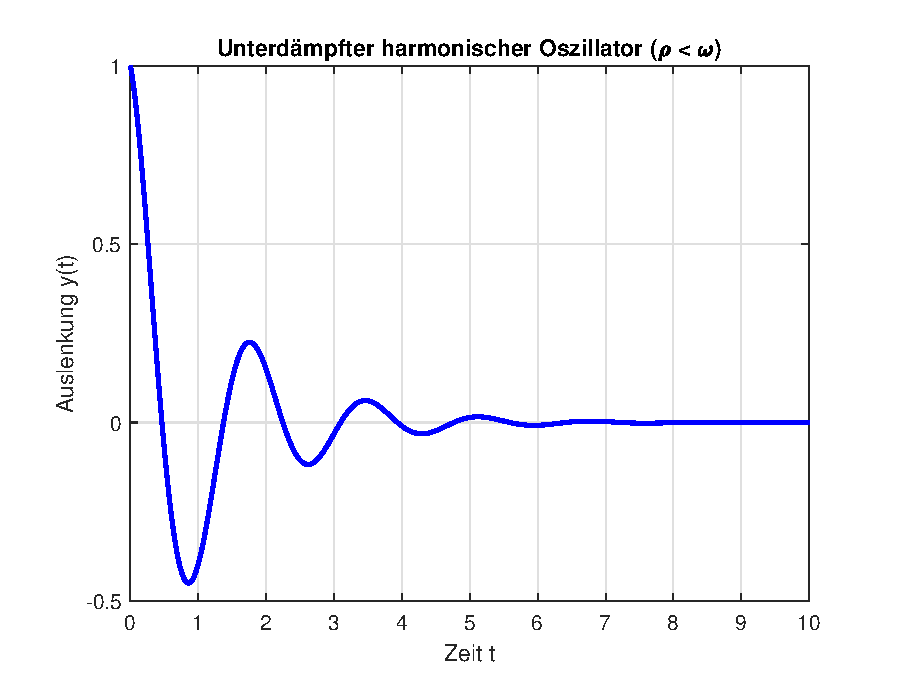
\includegraphics[width=0.6\textwidth]{unterdaempfterHarOszil.eps}
\end{figure}
}

\ErgebnisC{harmonischerOszillatorinhomogen}{
Fall 1: $y(t) = A\operatorname{e}^{(-\rho + \sqrt{\rho^2 - \omega^2})t} + B\operatorname{e}^{(-\rho - \sqrt{\rho^2 - \omega^2})t} + \frac{1}{2\sqrt{\rho^2 -\omega^2}}t \operatorname{e}^{(-\rho +  \sqrt{\rho^2 - \omega^2})t},$\\
Fall 2: $y(t) = (A+Bt) \operatorname{e}^{-\omega t} + \frac{1}{2}t^2 \operatorname{e}^{-\omega t},$\\
Fall 3: $y(t) = \operatorname{e}^{-\rho t}(A \cos(\sqrt{\omega^2 - \rho^2} t) + B \sin(\sqrt{\omega^2 - \rho^2} t))+\frac{1}{2}t\operatorname{e}^{-\rho t} \sin((\sqrt{\omega^2 - \rho^2})t).$
}



